Cross-Polytope LSH is one of the LSH family methods, it was proposed to estimate
Euclidean metric (\ref{subsect:euclidean_metric}) on a unit sphere, which also
corresponds to the Angular metric (\ref{subsect:angular_metric}). It relies on
the fact that elements that are close to each other (in the two previously
mentioned metrics) are more likely to be close to the same axis after applying a
random rotation. \citep{andoni_practicalsh_2015}

The figure \ref{fig:crosspolytope_example} show below shows how the
cross-polytope hashing works. We transform the data points to bring them to a
unit sphere, and then apply a random rotation to each one of them. The hash
value of each point will be the index of its nearest axis.

\begin{figure}[ht]
    \centering
    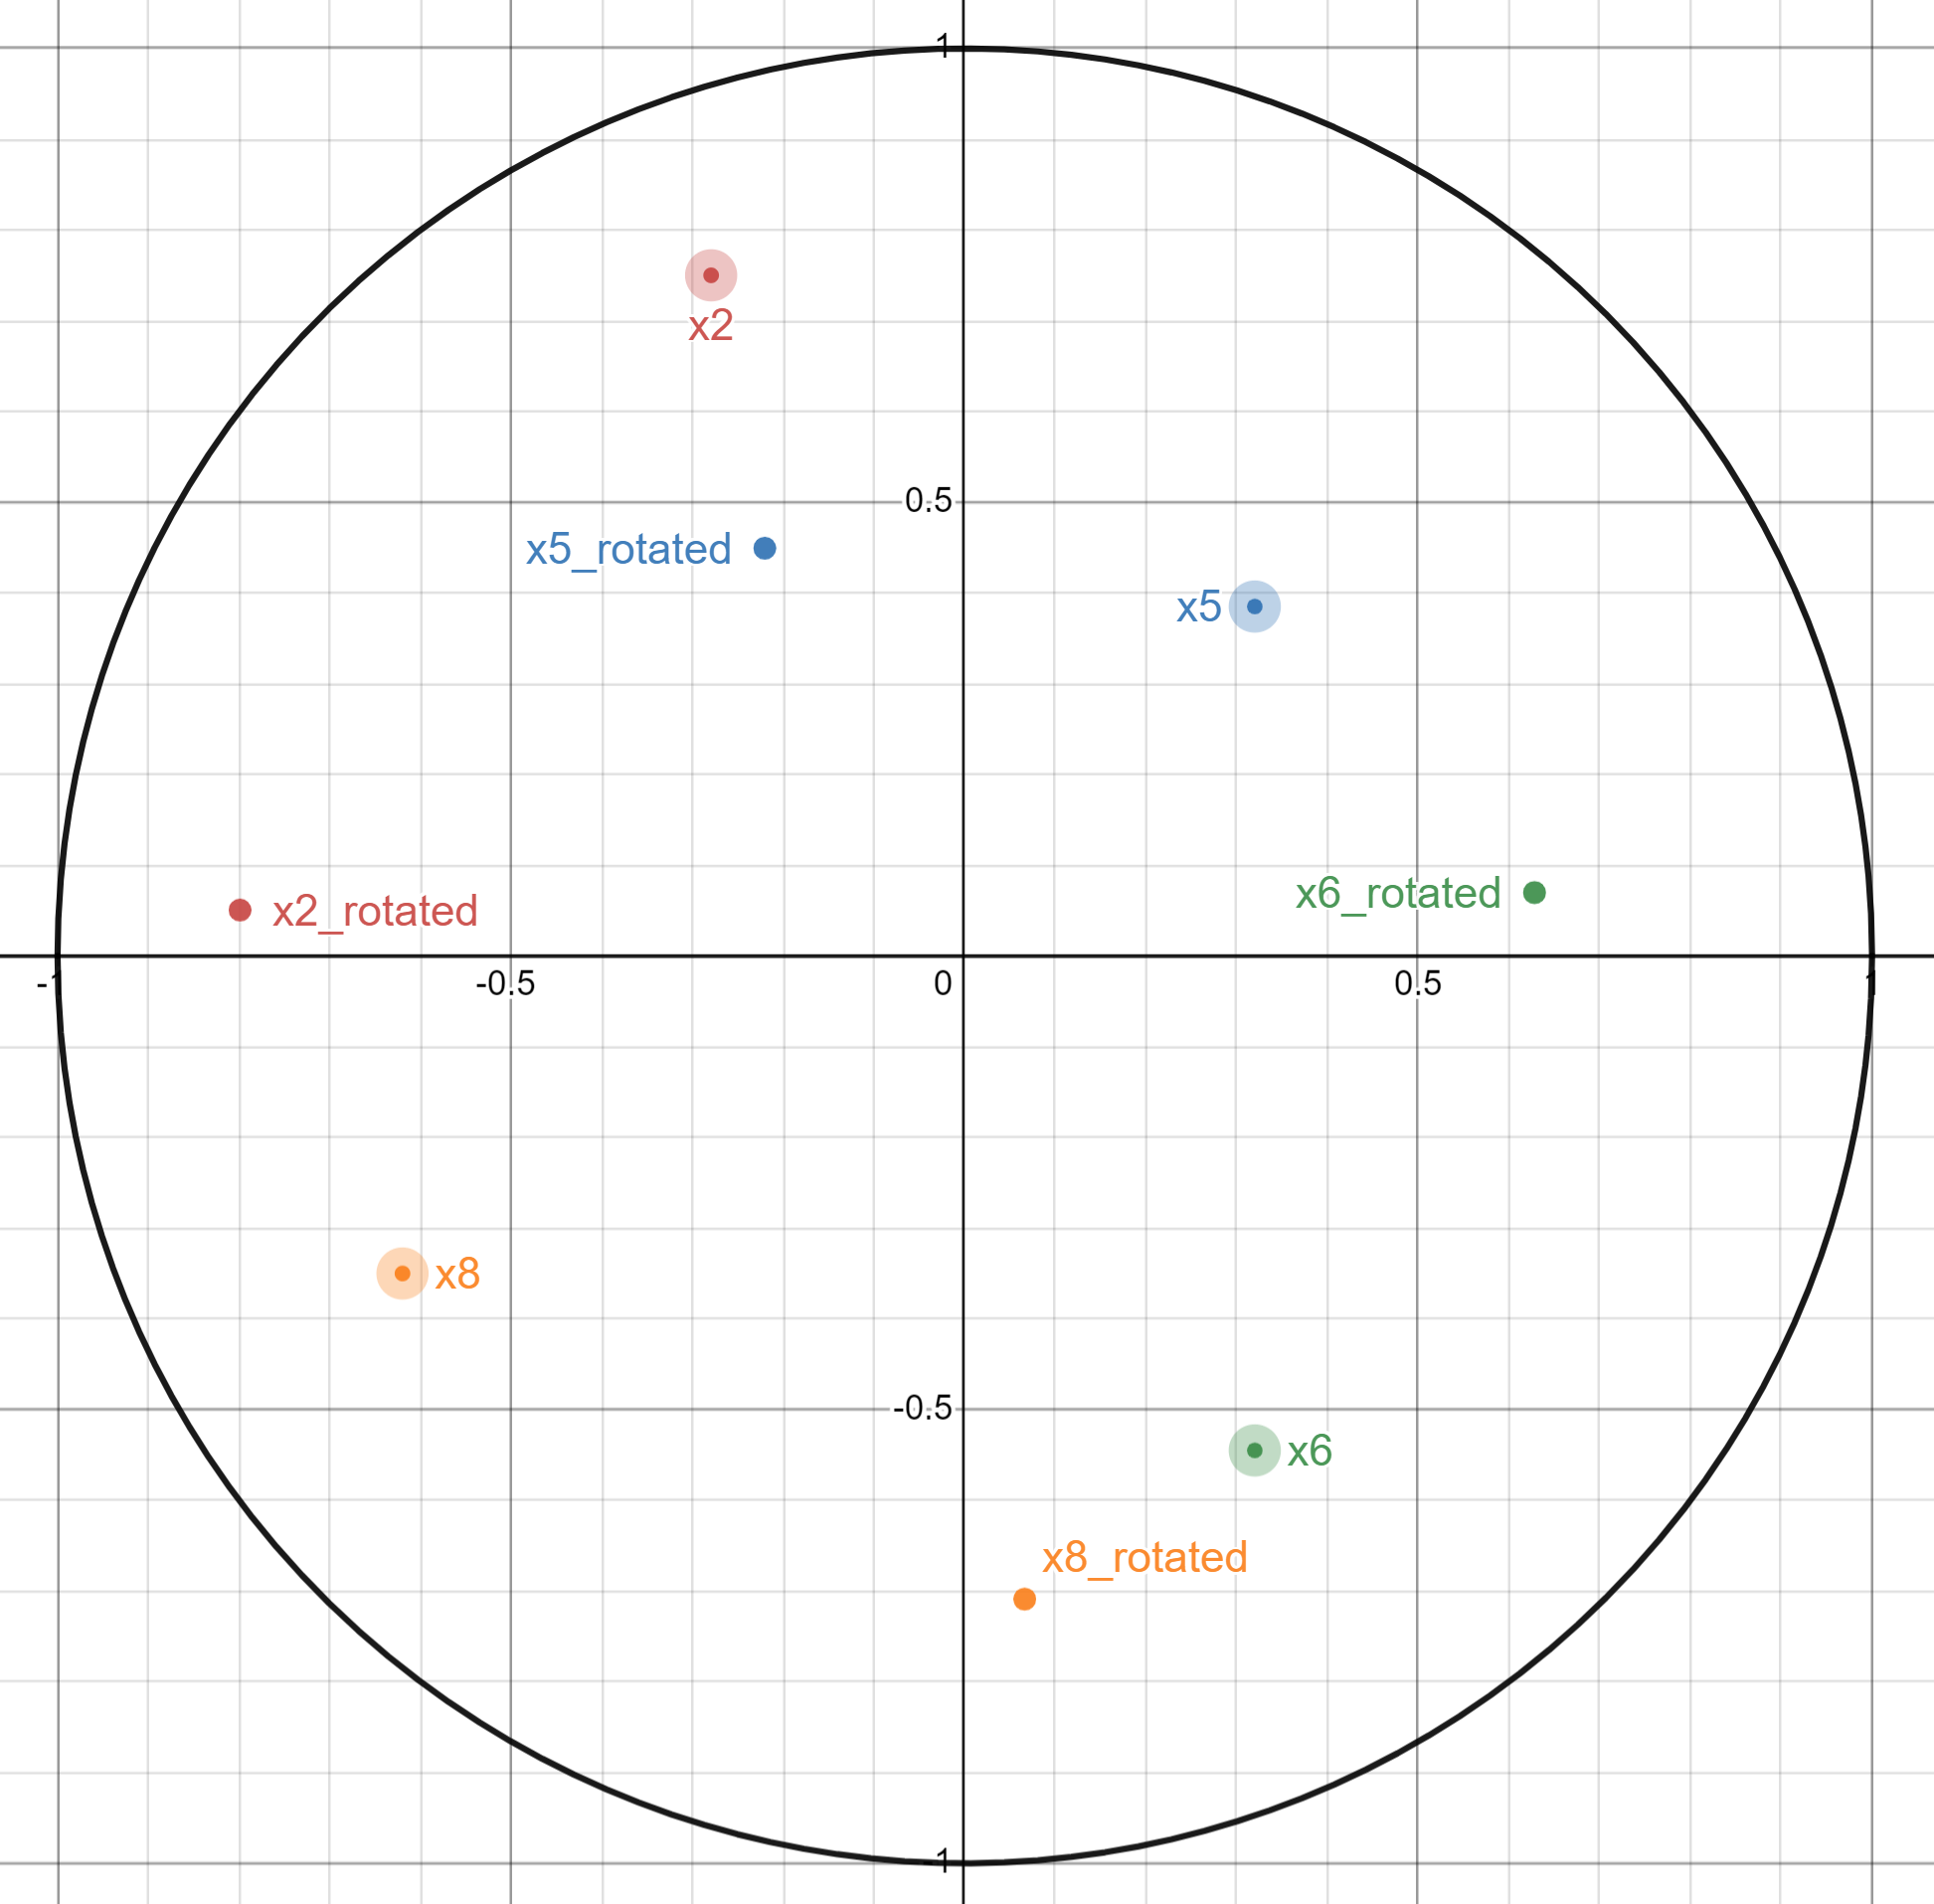
\includegraphics[height=0.4\textheight, width=\textwidth]{state_of_the_art/methods/cross-polyope.png}
    \caption{Cross-Polytope LSH example}
    \label{fig:crosspolytope_example}
\end{figure}

\subsubsection{Formulation}
Let $\mathcal{H}$ be a hash family for points on a unit sphere  $S^{d-1} \subset
    R^d$, and the random rotation matrix $A \in \mathbb{R}^{d*d}$ with i.i.d
gaussian entries. To get the hashing of a data point $x \in S^{d-1}$ with
cross-polytope LSH, we compute its normalized random rotation $y = \frac{A x
    }{\Vert{A x} \Vert} \in  S^{d-1}$ and then from basis vectors $\lbrace \pm
    e_i \; \vert 1 \leq i \leq d \rbrace$ the closest one.

This basis vector is the hash of $x$ with cross-polytope LSH. More formally we
write the hashing process as follow:
$$
    \mathcal{H}(x) = \arg \min_{u = \lbrace \pm e_i \rbrace} \lVert \frac{A x }{\Vert{A x} \Vert} - u \rVert
$$
This method has a time complexity of $O(d.n^\rho / p_1)$ and space complexity of
$O(n^{1 + \rho} / p_1 + dn)$, where $\rho = \frac{\log{1/
            p_1}}{\log{1/ p_2}}$ is the gap defined in \ref{sect:lsh_formulation}.
\citep{indyk_2000}

\subsubsection{Pseudo-random-rotation}
As described in \citep{andoni_practicalsh_2015}, the time complexity to apply a
random rotation (multiply $d * d$ matrix with a data point) is expensive, it is
at the order of $O(d^2)$ which will make the approach obsolete for large
dimensions. Empirically, it turns out that the pseudo-random rotation gives
similar results to the fully-random one. This pseudo-random rotation is given by
the following linear transformation:
$$
    x \mapsto HD_1HD_2HD_3x
$$
Where $H$ is the Hadamard matrix (\ref{subsubsect:hadamard_transform}), $D_1, D2,$
and $D_3$ are random diagonal matrices, whose the diagonal vector are randomly
picked from $\lbrace 1; -1 \rbrace$. To make the cross-polytope practical, we
use this linear transformation instead of using the random rotation.
$$
    \mathcal{H}(x) = \arg \min_{u = \lbrace \pm e_i \rbrace} \lVert \frac{HD_1HD_2HD_3x}{\Vert{HD_1HD_2HD_3x} \Vert} - u \rVert
$$

\subsubsection{Hadamard transform}
\label{subsubsect:hadamard_transform}
The Hadamard transform is an example of a generalized class of Fourier
transforms. It was named after the French mathematician Jacques Hadamard. This
transformation relies on a matrix (also named Hadamard matrix) to perform
orthogonal, symmetric, involutive, linear operation on $2^m$ real numbers.
(\href{https://www.quantiki.org/wiki/hadamard}{Quantiki}).

The Hadamard transforms are mainly used in signal decomposition applications, in
image processing, speech processing and power spectrum analysis.

a Hadamard matrix is a square matrix whose entries are either $+1$ or $-1$ and whose
rows are mutually orthogonal. $H_1 = 1$

$$
    H_2 =
    \begin{pmatrix}
        H_1 & H_1   \\
        H_1 & - H_1 \\
    \end{pmatrix}
$$

$$
    H_4 =
    \begin{pmatrix}
        H_2 & H_2   \\
        H_2 & - H_2 \\
    \end{pmatrix}
$$

This method can find its use in different applications like the comparison of
image feature vectors, speaker representations, and so on. Its main advantage is
that it come with theoretical guarantees to give a good approximation of the
angular and euclidean (on a unit sphere) metrics , and also with experimental
improvements on its complexity for the large datasets.
\citep{andoni_practicalsh_2015}
